\documentclass[11pt]{article}

\usepackage{times}
\usepackage{graphicx}
\usepackage{notes}
\usepackage{color, soul}
\usepackage{amsmath}

\textwidth=6.5in
\textheight=8.75in
\oddsidemargin=0.0in
\evensidemargin=0.0in
\topmargin=-0.5in

\usepackage{tikz}
\def\checkmark{\tikz\fill[scale=0.4](0,.35) -- (.25,0) -- (1,.7) -- (.25,.15) -- cycle;} 

\begin{document}
\thispagestyle{empty}

\renewcommand{\arraystretch}{1.5}



\lecture{CS 6300, Spring 2017}{HW01: Search}{Due: 24 January 2017}

Please use \LaTeX\ to produce your writeups. See the Homework Assignments 
page on the class website for details.

\begin{flushleft}
Name: \underline{Christopher Mertin}
\end{flushleft}

\section{Search}

Execute the following search algorithms on the graph below using
priority queues, by filling in the search table for each part.  (Not
all steps will necessarily be used.)  The arcs are bi-directional.

  \begin{center}
  \centerline{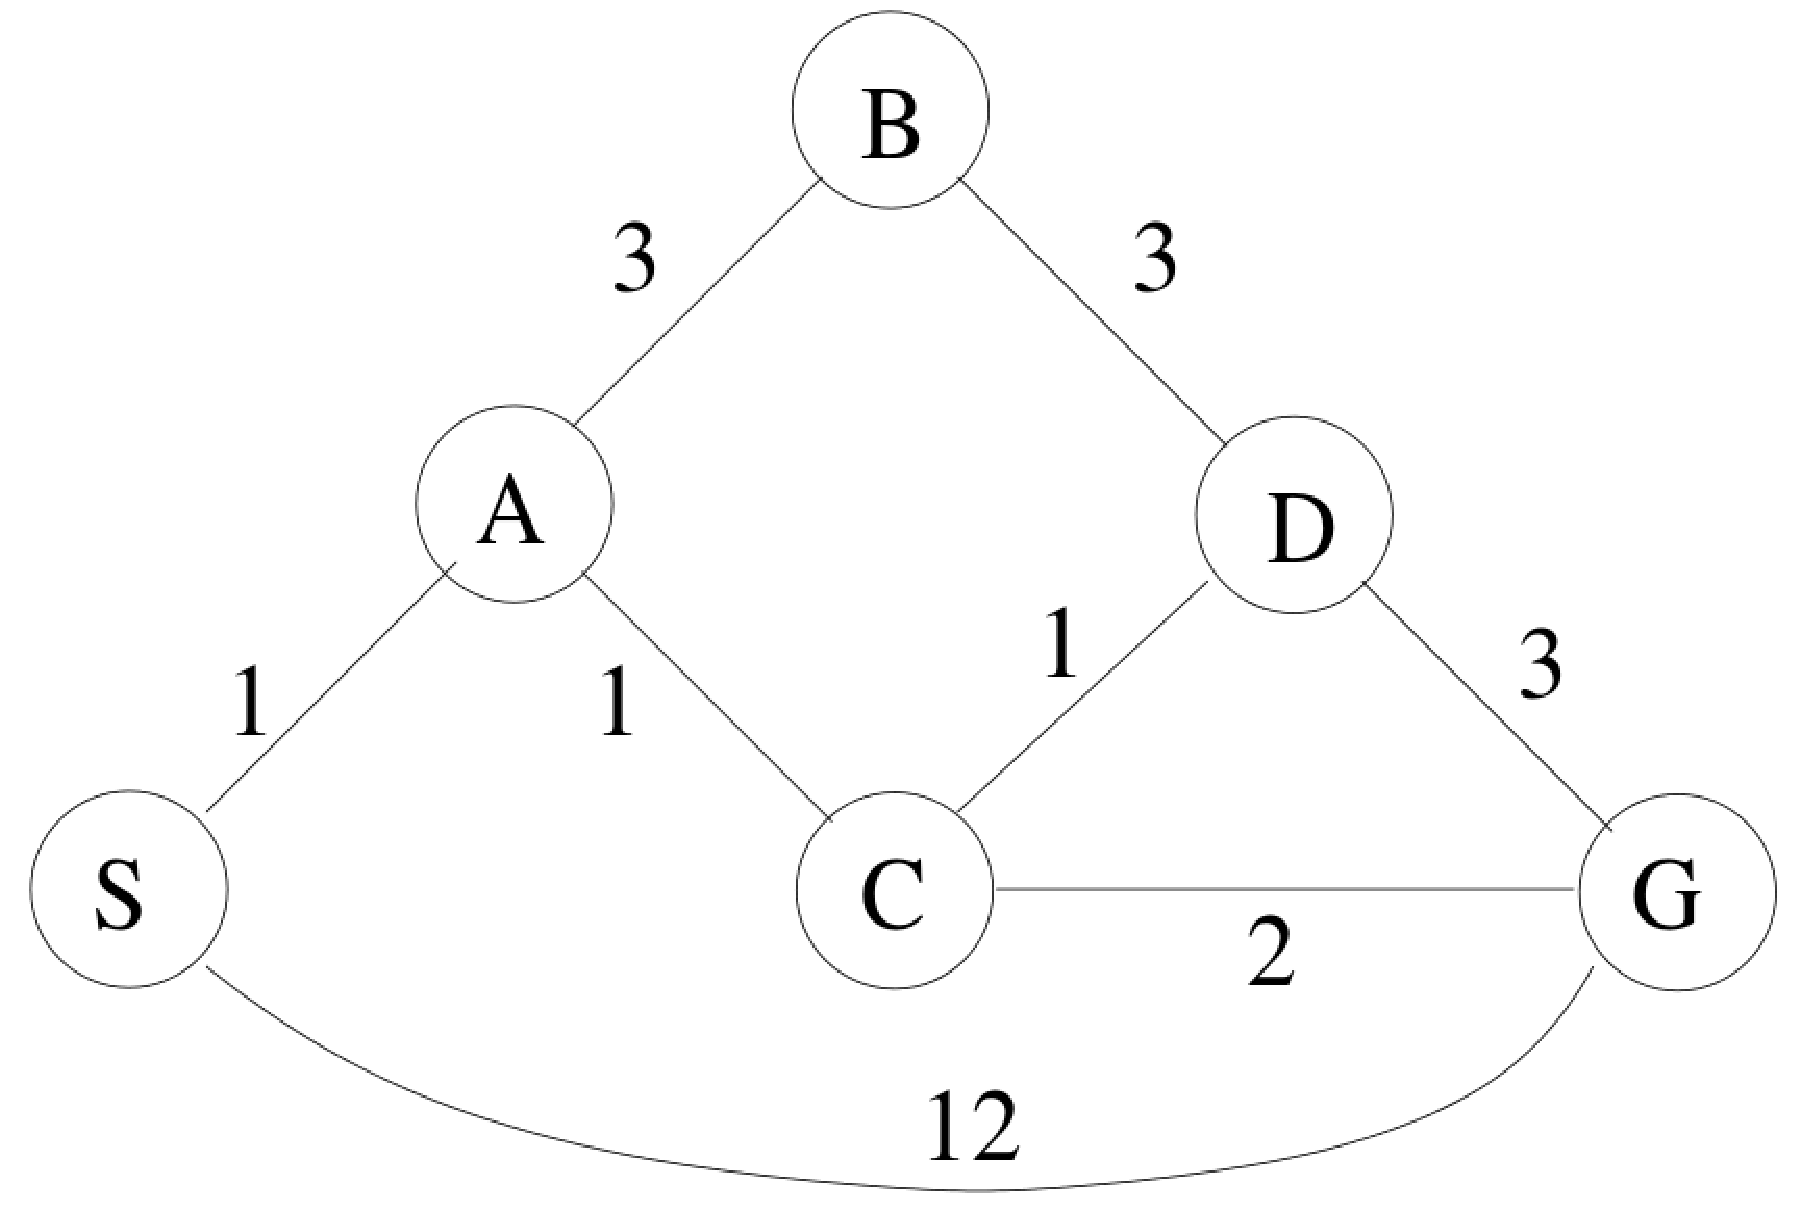
\includegraphics[width=3.5in]{diagram.pdf}}
  \end{center}

  \begin{description}

  \item[1 Breadth First Graph Search]

  \end{description}

    \begin{center}
    \begin{tabular}{|l|l|l|} \hline
    \bf Step & \bf Priority Queue  & \bf Expand \\ \hline
    1 & S & S \\ \hline
    2 & S-A, S-G & S-A\\ \hline
    3 & \textcolor{red}{\textbf{\hl{S-G}}}, S-A-B, S-A-C&  Found G\\ \hline
    4 & & \\ \hline
    5 & &  \\ \hline
    6 &  &  \\ \hline
    7 &   &  \\ \hline
    8 &   &  \\ \hline
    \end{tabular}
    \end{center}

\clearpage

  \begin{description}

  \item[2 Depth First Graph Search]

  \end{description}

    \begin{center}
    \begin{tabular}{|l|l|l|} \hline
    \bf Step & \bf Priority Queue  & \bf Expand \\ \hline
    1 & S & S \\ \hline
    2 & S-A, S-G  &  S-A\\ \hline
    3 & S-A-B, S-A-C, S-G  & S-A-B \\ \hline
    4 & S-A-B-D, S-A-C, S-G & S-A-B-D \\ \hline
    5 & \textcolor{red}{\textbf{\hl{S-A-B-D-G}}}, S-A-B-D-C, S-A-C, S-G  &  Found G\\ \hline
    6 &   &  \\ \hline
    7 &   &  \\ \hline
    8 &   &  \\ \hline
    \end{tabular}
    \end{center}

  \begin{description}

  \item[3 Uniform Cost Graph Search]

  \end{description}

    \begin{center}
    \begin{tabular}{|l|l|l|} \hline

    \bf Step & \bf Priority Queue  & \bf Expand \\ \hline
    1 & S & S \\ \hline
    2 & S-A, S-G & S-A \\ \hline
    3 & S-A-C, S-A-B, S-G & S-A-C \\ \hline
    4 & S-A-C-D, S-A-C-G, S-A-B, S-G  & S-A-C-D \\ \hline
    5 & \textcolor{red}{\textbf{\hl{S-A-C-G}}}, S-A-C-D-B, S-A-C-D-G, S-A-B, S-G  & Found G \\ \hline
    6 &   &  \\ \hline
    7 &   &  \\ \hline
    8 &   &  \\ \hline
    \end{tabular}
    \end{center}

  \begin{description}

\clearpage

  \item[4] Consider the heuristics for this problem shown in the table below.

     \begin{center}
     \begin{tabular}{|l|l|l|}\hline
     State & $h_1$ & $h_2$ \\ \hline
     S     & 5     & 4     \\ \hline
     A     & 3     & 2     \\ \hline
     B     & 6     & 6     \\ \hline
     C     & 2     & 1     \\ \hline
     D     & 3     & 3     \\ \hline
     G     & 0     & 0     \\ \hline
     \end{tabular}
     \end{center}

     \begin{enumerate}

     \item Is $h_1$ admissible?  If not, why? \\

       Not admissible as $h_{1}(S) = 5$, while the actual ``optimal cost'' from $S \rightarrow G$ is 4. It must be less than or equal to the actual cost to be admissible.

     \item Is $h_1$ consistent?  If not, why? \\

       To be consistent, $h(n) \leq c(n, a, n^{\prime}) + h(n^{\prime})$, where $a$ is any action and $n^{\prime}$ is every successor of $n$. Therefore, the estimated cost of reaching the goal from $n$ is no greater than the step cost of getting to $n^{\prime}$ plus the estimated cost of reaching the goal from $n^{\prime}$.

       Yes, it is consistent as we have 
       \begin{align*}
         h(S) &\leq c(S\rightarrow A) + c(A\rightarrow C \rightarrow G) + h(A)\\
         5 &\leq 1+1+2+2\\
         5 &\leq 6\;\checkmark
         \end{align*}

         This also holds true for all other nodes. 

     \item Is $h_2$ admissible?  If not, why? \\

       Not admissible as $h_{2}(A) = 2$, while the actual ``optimal cost'' from $A \rightarrow G$ is 3. It must be less than or equal to the actual cost to be admissible.

     \item Is $h_2$ consistent?  If not, why? \\

       Yes, it is consistent. An example node is as follows:
       \begin{align*}
         h(S) &\leq c(S\rightarrow A) + c(A\rightarrow C \rightarrow G) + h(A)\\
         4 &\leq 1+1+2+2\\
         4 &\leq 6\;\checkmark
         \end{align*}

         The rest of the nodes are left as an exercise to the reader.


     \end{enumerate}

  \end{description}

\end{document}
